\documentclass[11pt]{article}

\usepackage{ml5}

\newenvironment{exercise}{\item}{}
\newcommand{\solution}[1]{}

\newcommand{\w}{\omega}
\newcommand{\Int}{\mathbb{Z}}
\newcommand{\Compl}{\mathbb{C}}


\begin{document}

 \title{Математические основы алгоритмов, весна 2023 \\ Задание 2}
 \date{}
 \author{}
 \maketitle

\begin{enumerate}

\begin{exercise}
Докажите корректность схем битонного слияния и битонной сортировки, представленных в лекциях.
\end{exercise}

\begin{exercise}
Пусть имеется сеть сортировки. Останется ли она сетью сортировки, если

\begin{enumerate}
\item перевернуть ее диаграмму относительно вертикальной оси?
(при этом направление сортировки пар индивидуальными элементами сравнения не переворачивается)?

\solution{
True. Let $x_i$, $0 \leq i < n$, be the input to the modified network.
Consider $-x_{n-i}$, $0 \leq i < n$, as the input to the original network.
A comparator between a pair of lines $(i,j)$ exists in the modified network,
if and only if a comparator between the pair $(n-j,n-i)$ exists in the original network
at the same level.
Let a comparator in the top level of the modified network take inputs $x$, $y$;
then, the corresponding comparator in the original network takes inputs $-y$, $-x$ in that order.
We have $x < y$ if and only if $-y < -x$,
therefore one of the comparators swaps the inputs if and only if the other swaps.
Therefore, after passing through the first level of comparators,
we still have a value $x$ in line $k$ of the modified network,
if and only if we have value $-x$ in line $n-k$ of the original network.
By induction, this holds for every level in the network, including the output.
Let $y_i$, $0 \leq i < n$, be the output of the modified network.
Then, as shown above,
$-y_{n-i}$, $0 \leq i < n$, is the output to the original network.
Since the original network is a sorting network,
we have $-y_{n-i} < -y_{n-j}$ whenever $i < j$, 
therefore we have $-y_i < -y_j$ whenever $n-i < n-j$, 
i.e.\ $y_i > y_j$ whenever $i > j$.
Hence, the output of the modified network is sorted.
Since we assumed an arbitrary input, the modified network is a sorting network.
}

\item перевернуть ее диаграмму относительно горизонтальной оси?

\solution{
False. The picture on the left shows a sorting network, as proved in the lectures.
The picture on the right shows the same network, flipped around a horizontal axis.
It does not sort the input shown.
%
\begin{center}
%
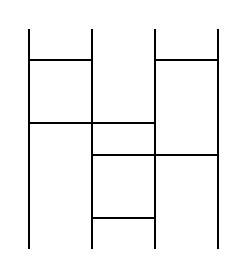
\begin{tikzpicture}[thick, x=0.8 cm, y=-0.8cm]
%
\draw \foreach \x in {0,...,3} {(\x,0) -- +(0,3.5)};
%
\draw
++(0,0.5) -- +(1,0) +(2,0) -- +(3,0)
++(0,1) -- +(2,0)  
++(0,0.5) +(1,0) -- +(3,0)
++(0,1) +(1,0) -- +(2,0);
%
\end{tikzpicture}
\qquad
%
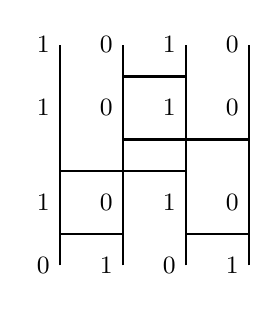
\begin{tikzpicture}[thick, x=0.8 cm, y=0.8cm]
%
\draw \foreach \x in {0,...,3} {(\x,0) -- +(0,3.5)};
%
\draw
++(0,0.5) -- +(1,0) +(2,0) -- +(3,0)
++(0,1) -- +(2,0)  
++(0,0.5) +(1,0) -- +(3,0)
++(0,1) +(1,0) -- +(2,0);
%
\draw
(0,3.5) node[left]{\small $1$}
(1,3.5) node[left]{\small $0$}
(2,3.5) node[left]{\small $1$}
(3,3.5) node[left]{\small $0$}
%
(0,2.5) node[left]{\small $1$}
(1,2.5) node[left]{\small $0$}
(2,2.5) node[left]{\small $1$}
(3,2.5) node[left]{\small $0$}
%
(0,1) node[left]{\small $1$}
(1,1) node[left]{\small $0$}
(2,1) node[left]{\small $1$}
(3,1) node[left]{\small $0$}
%
(0,0) node[left]{\small $0$}
(1,0) node[left]{\small $1$}
(2,0) node[left]{\small $0$}
(3,0) node[left]{\small $1$};
%
\end{tikzpicture}
%
\end{center}
}

\item добавить к сети произвольный элемент сравнения?

\solution{
False. The picture on the left shows a sorting network, as proved in the lectures.
The picture on the right shows the same network, 
with an extra comparator introduced in the second level between two middle lines.
It does not sort the input shown.
%
\begin{center}
%
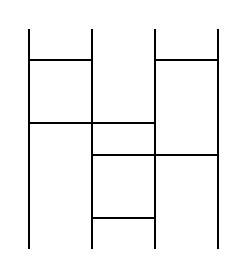
\begin{tikzpicture}[thick, x=0.8 cm, y=-0.8cm]
%
\draw \foreach \x in {0,...,3} {(\x,0) -- +(0,3.5)};
%
\draw
++(0,0.5) -- +(1,0) +(2,0) -- +(3,0)
++(0,1) -- +(2,0)  
++(0,0.5) +(1,0) -- +(3,0)
++(0,1) +(1,0) -- +(2,0);
%
\end{tikzpicture}
\qquad
%
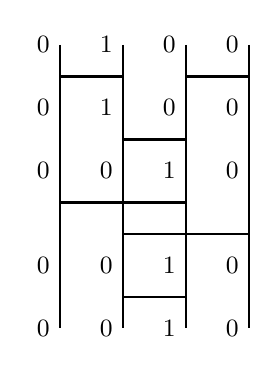
\begin{tikzpicture}[thick, x=0.8 cm, y=-0.8cm]
%
\draw \foreach \x in {0,...,3} {(\x,0) -- +(0,4.5)};
%
\draw
++(0,0.5) -- +(1,0) +(2,0) -- +(3,0)
++(0,1) +(1,0) -- +(2,0)
++(0,1) -- +(2,0)
++(0,0.5) +(1,0) -- +(3,0)
++(0,1) +(1,0) -- +(2,0);
%
\draw
(0,0) node[left]{\small $0$}
(1,0) node[left]{\small $1$}
(2,0) node[left]{\small $0$}
(3,0) node[left]{\small $0$}
%
(0,1) node[left]{\small $0$}
(1,1) node[left]{\small $1$}
(2,1) node[left]{\small $0$}
(3,1) node[left]{\small $0$}
%
(0,2) node[left]{\small $0$}
(1,2) node[left]{\small $0$}
(2,2) node[left]{\small $1$}
(3,2) node[left]{\small $0$}
%
(0,3.5) node[left]{\small $0$}
(1,3.5) node[left]{\small $0$}
(2,3.5) node[left]{\small $1$}
(3,3.5) node[left]{\small $0$}
%
(0,4.5) node[left]{\small $0$}
(1,4.5) node[left]{\small $0$}
(2,4.5) node[left]{\small $1$}
(3,4.5) node[left]{\small $0$};
%
\end{tikzpicture}
\qquad

\end{center}
}

\end{enumerate}
\end{exercise}

\begin{exercise}

\emph{Сетью транспозиции} называется сеть сравнения, 
в диаграмме которой все попарные сравнения производятся между соседними проводами.

\begin{enumerate}

\item Докажите, что если сеть транспозиции на $n$ входах является сетью сортировки,
то в ней не менее $\binom{n}{2}$ элементов сравнения.

\solution{Knuth v3 5.3.4 ex 35:
рассмотреть число инверсий исходной перестановки}

\item Докажите, что если сеть транспозиции на $n$ входах сортирует последовательность
$(n, n-1, \ldots 2, 1)$ (то есть последовательность, отсортированную по убыванию),
то она является сетью сортировки.

\solution{Knuth v3 5.3.4 ex 36:
от противного. Пусть пара выходов не отсортирована, wlog 1, 0.
Рассмотрим пути.
Поменяем вход на 1111000.}

\end{enumerate}

\end{exercise}

\begin{exercise}
Ответьте на вопросы упражнения 2 при условии, что упоминаемая в них сеть является сетью транспозиции.

\solution{

а: тривиально

b: A minimal transposition sorting network is a shortest path from 12...n to n...21 in the Cayley graph 
of the symmetric group generated by adjacent transpositions.

Геометрия графа Кэли: пермутоэдр (перестановочный многогранник)

Все вершины лежат на $n-2$-мерной сфере (сумма координат и квадратов координат --- константа)

Недавно доказана гипотеза: случайная сортирующая сеть транспозиций в пределе стремится 
к большой полуокружности на этой сфере.

c: сортируем 654321. Пара переставилась лишним компаратором - дальше только лучше, сортирует.
}

\end{exercise}

\begin{exercise}

\emph{Правильная скобочная последовательность} определяется рекурсивно:
это либо пустая последовательность, либо последовательность `($S$)', либо последовательность `$ST$',
где $S$, $T$ --- правильные скобочные последовательности.
Например, скобочные последовательности `(((())))', `()(())()((()))', `' --- правильные, 
а последовательности `)(', `(()))' --- неправильные. 
Опишите эффективную параллельную схему распознавания правильных скобочных последовательностей.

\solution{Префиксные суммы на значениях $-1$, $1$.}

\end{exercise}

\begin{exercise}
В коде на языке Python, комментарий состоит из символа `\texttt{\#}' 
и всех следующих за ним символов, вплоть до конца строки.
(Комментарий может, в числе прочих, содержать произвольное количество символов `\texttt{\#}').
Задан массив из $n$ символов, содержащий код на Python;
в нем концы строк обозначены специальным символом `$\hookleftarrow$', 
ограничения на длину строки отсутствуют. 
Опишите эффективную параллельную схему, заменяющий все символы комментариев на пробелы.

\solution{
Let $b_i$ be a Boolean value indicating whether character $a_i$ is part of a comment.
We have
%
\begin{gather*}
%
b_i \equiv (a_i = \text{`\texttt{\%}'}) \lor ((a_i \neq \mathit{eol}) \land b_{i-1})
%
\end{gather*}
%
In this form, the problem is an instance 
of a generic first-order linear recurrence defining a Boolean array $b$
with coefficients evaluated as Boolean expressions 
$a_i = \text{`\texttt{\#}'}$, $a_i \neq \mathit{eol})$, 
where disjunction $\lor$ plays the role of addition,
and conjunction $\land$ that of multiplication.
Since both these operations are associative and $\land$ distributes over $\lor$,
we can apply the reduction to prefix sums over $2 \times 2$ matrix multiplication
shown in lectures to obtain an efficient circuit for this problem.
}

\end{exercise}

\begin{exercise}
Система линейных уравнений $Ax = b$ задана $n \times n$ матрицей $A$ и $n$-вектором $b$.
Матрица $A$ является \emph{трехдиагональной}, то есть $a_{ij}=0$ для всех $i$, $j$, где $\abs{i-j}>1$.
Опишите эффективную параллельную схему для решения такой системы
%
\begin{enumerate}
%
\item предполагая, что $a_{ij} \neq 0$ при $\abs{i-j} \leq 1$
\item* в общем случае
%
\end{enumerate}
%
Предполагается, что решение существует и единственно, и что все вычисления точные.

\solution{
Generalised linear recurrence on matrices}

\end{exercise}

\begin{exercise}
Опишите эффективный параллельный алгоритм для быстрого преобразования Фурье в произвольном кольце $R$
(удовлетворяющем условиям существования DFT):
%
\begin{enumerate}
%
\item как схему с элементарными операциями сложения и умножения в $R$;
%
\item в модели BSP с оптимальной трудоемкостью и коммуникацией, 
и минимально возможным количеством синхронизаций;
при этом можно предположить, что степень преобразования $n$ достаточно велика 
по сравнению с количеством процессоров $p$.
%
\end{enumerate}

\solution{
Пусть $n \geq p^2$.
Разрезаем граф посередине. Верхняя и нижняя половины обе распадаются на $\sqrt n \geq p$ 
независимых подграфов размера $\sqrt n$.
Распределяем их равномерно между процессорами.
Одна синхронизация посередине.}

\end{exercise}

\begin{exercise}*
Опишите эффективный параллельный алгоритм для сортировки массива из $n$ элементов 
произвольного линейно упорядоченного множества
с элементарной операцией сравнения двух элементов,
в модели BSP с оптимальной трудоемкостью и коммуникацией, 
и минимально возможным количеством синхронизаций;
при этом можно предположить, что размер массива $n$ достаточно велик 
по сравнению с количеством процессоров $p$.
\end{exercise}

\end{enumerate}

\end{document}
